\documentclass[thesis]{subfiles}

\begin{document}

\section{Figures and labels}
\label{sec:5} % might not be such an intuitive label... what if we change the order so it is no longer section 5? You should label according to content, so you don't need to remember the number of the section about figures and labels and are not confused when you decide to change the order of sections.
You probably want to include some figures in your thesis, either to illustrate an abstract idea or to present graphs or other results you obtained with your data.

In this section we give some code (see the source code below) you can use and adapt this yourself.
We do this in the figure environment (needs graphicx package).

First we give a refresher:
\begin{table}[h] % as you can see, the same placement letters
			  	 % are also used for tables
	\centering
	\begin{tabular}{lll}
		h &	here    & Place figure {ABOUT} here in the text. \\
		t & top     & Place figure on the top of the page. \\
		b & bottom  & Place figure at the bottom of the page. \\
		p &	page    & Place figure on a seperate page for figures. \\
		! &	        & You can put this command after one of the above  \\ 
		&         & to override the intern parameters for finding \\
		&         & a good position. \\
		H & HERE    & Place figure exactly {HERE} in the document. \\
		&         & Looks a lot like the h! command.
	\end{tabular}
	\caption{Reference table for figure placing.}
	\label{tab:location}
\end{table}

In square brackets we have letters indicating where to put the figure, see \ref{tab:location}.
It does not matter in which order you use h, p, t, b or !, \LaTeX{} uses the following order: 
\begin{itemize}
	\item Looks whether there is an h. If there is, it tries to place the figure immediately.
	\item If that did not work and there is a t, tries to place figure at the top of the page.
	\item Then it tries the b for the bottom of the page.
	\item If it still did not work yet, the figure is placed on hold, to be placed when/where you start on a new page. For example, you could use the command \textbackslash clearpage.
\end{itemize}

You can refer to figures in advance, since Figure \ref{fig:asbak} is on page \pageref{fig:asbak}, note your labelname is your own to choose and does not show up in the pdf, however, you might want to stick to some logic and for example take into account what it is you are refering to, eg use fig, tab, sec if you label a figure, table or section (see table \ref{tab:conventions} on page \pageref{tab:conventions}). It makes more sense refering to table \ref{tab:location} instead of simply refering to \ref{tab:location} or \ref{sec:5} since there may exist a section, table and figure of that number. Try what the command \textbackslash autoref can do for you in this regard!

Also note you can number figures continuously (the first picture in your document 1, second 2, etc.), or per section (then you get the third figure in section 2 labeled as 2.3). See the preamble (around lines 100) for this (it also works for equations).

\begin{figure}[htbp] 
	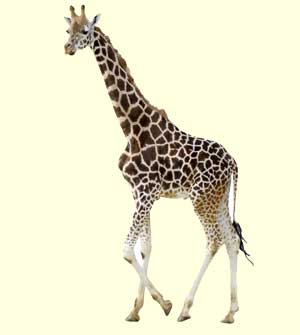
\includegraphics[width=0.9\linewidth]{Giraffe_klein.jpg}
	\caption{My plot}
	\label{fig:myPlot}
\end{figure}

\begin{figure}[h!]
    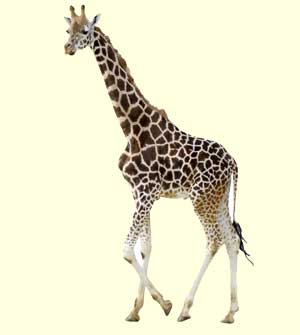
\includegraphics[height = 10cm, width = 4cm]{Giraffe_klein.jpg}
    \caption{This is an African animal}
    \label{fig:Lang}
\end{figure}

\begin{figure}[b!]
    
\includegraphics[scale = 0.9, angle = 31.4159]{uulogoEN.png}
    \caption{We can even rotate pictures}
    \label{fig:asbak}
\end{figure}
\clearpage

We can also make subfigures, here we have figures \ref{fig:coulors} and \ref{fig:littleanimal} inside figure \ref{fig:subfigures}
\begin{figure}
	\begin{subfigure}[b] 	% Align side-by-side on bottom 
							%	(other alignments are also possible)
		{0.45\textwidth}    % Width: half page width with some space between
		\centering
		
\includegraphics[width=\linewidth]{ibavlag.jpg}
		\caption{colours}
		\label{fig:coulors}
	\end{subfigure}
	\begin{subfigure}[b]
		{0.45\textwidth}
		\centering
		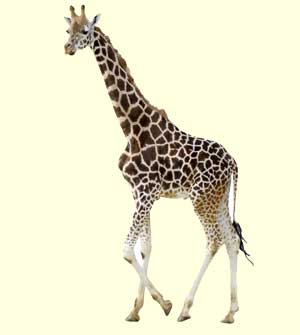
\includegraphics[width=\linewidth]{Giraffe_klein.jpg}
		\caption{giraffe}
		\label{fig:littleanimal}
	\end{subfigure}	
	\caption{two figures next to each other, left colours, right a giraffe}
	\label{fig:subfigures}
\end{figure}
		
And you might want to make a \dots 
\listoffigures
Note subfigures are not included in this list!

You can also make a \dots  
\listoftables

\begin{table}[b] % Note this table moves up if you remove [b]
	\centering
	\begin{tabular}{c|l}
		eq:&	equation \\ 
		fig:&	figure \\
		tab:&	table \\
		chap: &	chapter \\
		sec:&	section \\
		subsec:&	subsection \\
		itm:&	enumerated list item \\
		app:&	appendix subsection
	\end{tabular}
	\caption{Some conventions in labeling}
	\label{tab:conventions}
\end{table}
\end{document}